\chapter{Task 3}
\UseRawInputEncoding
\begin{parlist}
 \item korrigieren() should look at the solution for each question and give it points depending on how correct/incorrect it is.

 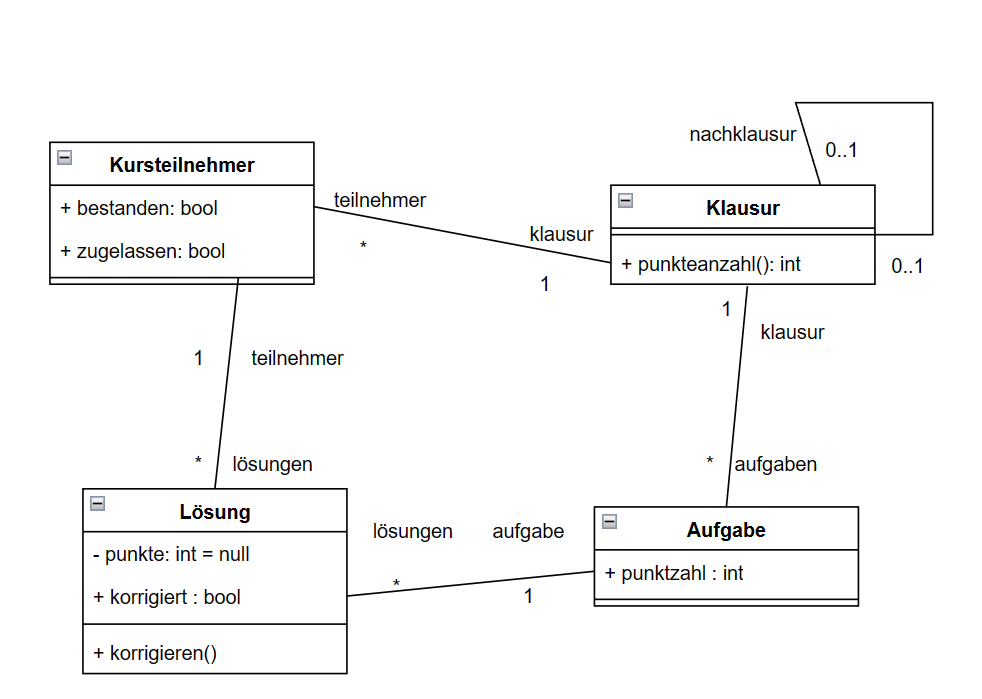
\includegraphics[width=\textwidth]{Immagini/aufg3}

 \item constraints for korrigieren with only one run per instance
 \begin{lstlisting}[language=OCL,frame=trBL]
context Loesung::korrigieren() pre: aufgabe != null
context Loesung::korrigieren() pre: teilnehmer != null
context Loesung::korrigieren() pre: not korrigiert
context Loesung::korrigieren() post: korrigiert = true
context Loesung::korrigieren() post: punkte <= aufgabe.punktzahl
context Loesung::korrigieren() post: punkte >= 0
\end{lstlisting}

 \item constraints for korrigieren with multiple runs per instance
\begin{lstlisting}[language=OCL, frame=trBL]
context Loesung::korrigieren() pre: aufgabe != null
context Loesung::korrigieren() pre: teilnehmer != null
context Loesung::korrigieren() post: korrigiert = true
context Loesung::korrigieren() post: punkte <= aufgabe.punktzahl
context Loesung::korrigieren() post: punkte >= 0
\end{lstlisting}

 \item constraints for punkteanzahl()
\begin{lstlisting}[language=OCL, frame=trBL]
context Klausur::punkteanzahl post: result = aufgaben->collect(punktzahl)->sum()
\end{lstlisting}

\end{parlist}

